%%%%%%%%%%%%%%%%%%%%%%%%%%%%%%%%%%%%%%%%%%%%%%%%%%%%%%%%%%%%%%%%%%%%%%%%%%%%%%%%%%%%
% source1 : http://sdz.tdct.org/sdz/creez-vos-diaporamas-en-latex-avec-beamer.html
% source2 : https://deic.uab.cat/~iblanes/beamer_gallery/index_by_theme_and_color.html
% logo https://latex-beamer.com/tutorials/logo-beamer/
%%%%%%%%%%%%%%%%%%%%%%%%%%%%%%%%%%%%%%%%%%%%%%%%%%%%%%%%%%%%%%%%%%%%%%%%%%%%%%%%%%%%
\documentclass[10pt]{beamer}
%%%%%%%%%%%%%%%%%%%%%%%%%%%%%%%%%%%%%%%%%%%%
%\usepackage[frenchb]{babel}
\usepackage[french]{babel}
\usepackage[autolanguage]{numprint} % for the \nombre command
%====================================================================
% pour les dessins 
\usepackage{tikz} 

% Set page size and margins
% Replace `letterpaper' with `a4paper' for UK/EU standard size
%\usepackage[letterpaper,top=2cm,bottom=2cm,gauche=3cm,droit=3cm,marginparwidth=1.75cm]{geometry}

%====================================================================
%les maths 
%\usepackage{graphicx}
%\usepackage[colorlinks=true, allcolors=blue]{hyperref}
%\usepackage[pdfpagelabels, allcolors=blue, colorlinks=true]{hyperref}

\usepackage{hyperref}
\hypersetup{colorlinks=true,linkcolor=blue,urlcolor=blue,citecolor=blue,anchorcolor=blue}


\usepackage{amsmath, amsthm, amssymb}
%\usepackage{amsthm,amsmath}


% incrementation 
\newtheorem{prop}{Proposition}
\renewcommand{\qedsymbol}{$\blacktriangledroit$}

%\newtheorem{theorem}{Theorem} %https://www.overleaf.com/learn/latex/Theorems_and_proofs
%===============================================================
\newcommand{\gatherblock}[2][]{\begin{gather*}\tcboxmath[#1]{#2}\end{gather*}}


%===============================================================
\usepackage{algorithm}
\usepackage{algpseudocode}

\newcommand{\algorithmicinput}{\textbf{Entrée:}}
\newcommand{\INPUT}{\item[\algorithmicinput]}
\newcommand{\algorithmicoutput}{\textbf{Sortie:}}
\newcommand{\OUTPUT}{\item[\algorithmicoutput]}

%\newcommand{\algorithmiccomment}[1]{\{#1\}}
\renewcommand{\algorithmicend}{\textbf{Fin}}

\renewcommand{\algorithmicif}{\textbf{Si}}
\renewcommand{\algorithmicthen}{\textbf{Alors}}
\renewcommand{\algorithmicelse}{\textbf{Sinon}}
\newcommand{\algorithmicelsif}{\algorithmicelse\ \algorithmicif}
\newcommand{\algorithmicendif}{\algorithmicend\ \algorithmicif}
\renewcommand{\algorithmicfor}{\textbf{Pour}}
\renewcommand{\algorithmicforall}{\textbf{Pour tous}}
\renewcommand{\algorithmicdo}{\textbf{Faire}}
\newcommand{\algorithmicendfor}{\algorithmicend\ \algorithmicfor}
\renewcommand{\algorithmicendfor}{\textbf{Fin pour}}
\renewcommand{\algorithmicwhile}{\textbf{Tanque}}
%=============================


\usepackage{caption}
%=====================================================================
\DeclareUnicodeCharacter{2212}{-}
%====================================================================
% ne pas compter certains slides
% soure : 
% Custom numbering for the footline
\setbeamertemplate{footline}{%
  \raisebox{5pt}{%
    \makebox[\paperwidth]{%
      \hfill\makebox[10pt]{%
        \footnotesize\insertframenumber
      }
    }
  }
}
%====================================================================
% Author-year citation in LaTeX
% source : http://merkel.texture.rocks/Latex/natbib.php
\usepackage[angle, comma, numbers, authoryear, colon]{natbib}

\usepackage{filecontents}
%====================================================================

%%%%%%%%%%%%%%%%%%%%%%%%%%%%%%%%%%%%%%%%%%%%
\setbeamertemplate{navigation symbols}{} % Supprimer la navigation
\usetheme{CambridgeUS} %Theme
\usecolortheme{dolphin} 
\usefonttheme{default}
%\usetheme{EastLansing}
%%%%%%%%%%%%%%%%%%%%%%%%%%%%%%%%%%%%%%%%%%%%
% definir la couleur du titre http://sdz.tdct.org/sdz/creez-vos-diaporamas-en-latex-avec-beamer.html#Modesdecouleurs
\definecolor{myblue1}{RGB}{188,188,228} 

%%%%%%%%%%%%%%%%%%%%%%%%%%%%%%%%%%%%%%%%%%%%
%https://tex.stackexchange.com/questions/151306/beamer-titlepage-picture
\addtobeamertemplate{title page}{
\includegraphics[scale=.05]{logoUmons.png} \hfill 
\includegraphics[scale=0.19]{index.png} \\[.2cm]}{}
\setbeamercolor{title}{bg=myblue1,fg=black}

%%%%%%%%%%%%%%%%%%%%%%%%%%%%%%%%%%%%%%%%%%%%
% set captions of figure with numbers, 
% source : https://latex-beamer.com/tutorials/beamer-figure/
\setbeamertemplate{caption}[numbered]

%%%%%%%%%%%%%%%%%%%%%%%%%%%%%%%%%%%%%%%%%%%%
% Definir la couleur des blocks, 
% source:  https://perso.crans.org/besson/internship-mva-2016/slides/naereenbeamer.sty
\setbeamercolor{block body}{bg=normal text.bg!90!black}
\setbeamercolor{block title}{use={normal text,example text},bg=myblue1}

%%%%%%%%%%%%%%%%%%%%%%%%%%%%%%%%%%%%%%%%%%%%
% https://tex.stackexchange.com/questions/30461/beamer-nonumber-equivalent-for-slides
% Pour ne pas numéroté certains pages
%%%%%%%%%%%%%%%%%%%%%%%%%%%%%%%%%%%%%%%%%%%%
% How to change the color of \href links... for real https://tex.stackexchange.com/questions/13423/how-to-change-the-color-of-href-links-for-real
\definecolor{links}{HTML}{2A1B81}
\hypersetup{colorlinks,linkcolor=,urlcolor=links}

%\setbeamertemplate{footline}[page number]{}
%%%%%%%%%%%%%%%%%%%%%%%%%%%%%%%%%%%%%%%%%%%%%%%%%%%%%%%%%%%%%%%%%%

\title[Graphe planaire représentation straight line]{Représentation "Straight line" d'un graphe planaire \\ par l'algorithme Shift method}
\author[Youness KAZZOUL]{ 
	Directeur : M\textsuperscript{r} Jef \textsc{WIJSEN} \\[0.1cm] 
	Présenté par Youness \textsc{KAZZOUL} \\[1cm] 
	Université de Mons - Faculté des Sciences}
\date[Umons - 2023]{Umons - 2023}
%%%%%%%%%%%%%%%%%%%%%%%%%%%%%%%%%%%%%%%%%%%%%%%%%%%%%%%%%%%%%%%%%%
\DeclareUnicodeCharacter{2212}{-}
%%%%%%%%%%%%%%%%%%%%%%%%%%%%%%%%%%%%%%%%%%%%%%%%%%%%%%%%%%%%%%%%%%

\begin{document}	

\begin{frame}[plain,noframenumbering]
 \maketitle	
\end{frame}

%%%%%%%%%%%%%%%%%%%%%%%%%%%%%%%%%%%%%%%%%%%%%%%%%%%%%%%%%%%%%%%%%%

\begin{frame}[plain,noframenumbering]{Table des matières}
\setbeamertemplate{section in toc}[sections numbered]
\tableofcontents%[hideallsubsections]
~\end{frame}

%%%%%%%%%%%%%%%%%%%%%%%%%%%%%%%%%%%%%%%%%%%%%%%%%%%%%%%%%%%%%%%%%%
%%%%%%%%%%%%%%%%%%%%%%%%%%%%%%%%%%%%%%%%%%%%%%%%%%%%%%%%%%%%%%%%%%

\section[Introduction]{Introduction}
\begin{frame}{Introduction}
\begin{columns}
\begin{column}{0.3\textwidth}
    \centering
    \begin{block}{}
    - 2-connexe
    \end{block}
    \begin{block}{}    
    - Triangulé \\ [.5cm]    
    \end{block}
    \begin{block}{}        
    - Planaire maximal 
    \end{block}
\end{column}
    
    \begin{column}{0.6\textwidth}
    
	\begin{figure}	
	\centering	
	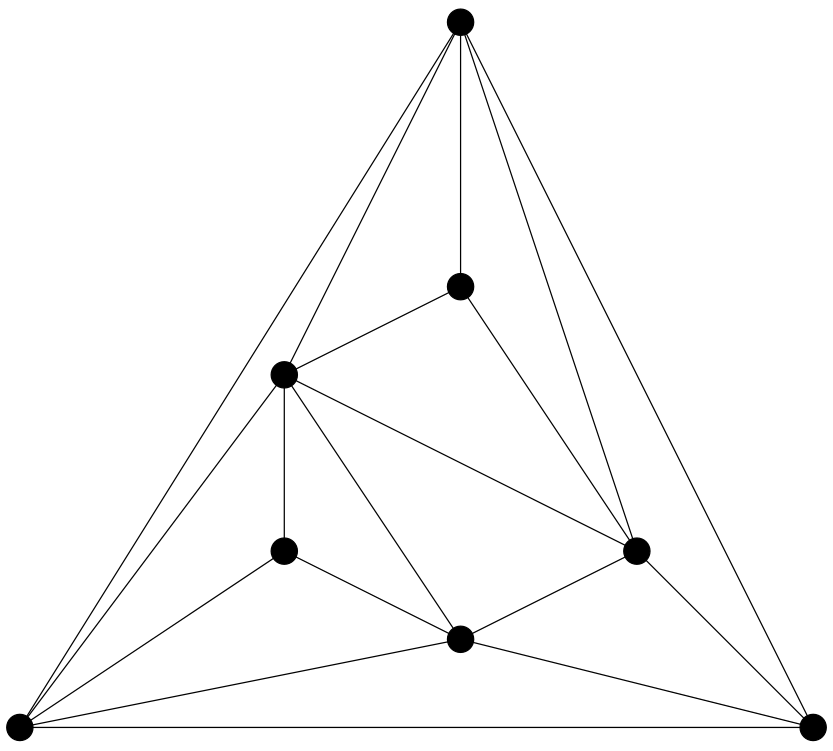
\includegraphics[height=0.5\textheight]{lineDroite.png}\\[.1cm]
    \caption[caption]{Dessin en ligne droite d’un graphe planaire.  \\\vspace*{0.3cm} Source: Repéré sur le document \citeauthor{TakaoSaidur}}	
	\end{figure}	
    \end{column}
\end{columns}  

\end{frame}

%%%%%%%%%%%%%%%%%%%%%%%%%%%%%%%%%%%%%%%%%%%%%%%%%%%%%%%%%%%%%%%%%%
%%%%%%%%%%%%%%%%%%%%%%%%%%%%%%%%%%%%%%%%%%%%%%%%%%%%%%%%%%%%

\section[Complexité]{Complexité}

\begin{frame}
	\frametitle{Complexité}
\begin{block}{Théorème \cite{FraysseixPachPollack} \cite{ChrobakPayne}} 
 Soit $G$ un graphe plan maximal avec $n$ sommets. Shift method calcule un dessin planaire en lignes droites de $G$ sur une grille de $(2n - 4) × (n - 2)$ en temps et en espace $\mathcal{O}(n)$ .
\end{block}

\begin{minipage}{0.4\textwidth}
    \begin{block}{}
        $1^{er}$  phase prend $\mathcal{O}(n)$ \\
        $2^{eme}$ phase prend $\mathcal{O}(d(v_k))$ \\ 
        $3^{eme}$ phase prend $\mathcal{O}(n)$
    \end{block}
\end{minipage}
        
\end{frame}	
%%%%%%%%%%%%%%%%%%%%%%%%%%%%%%%%%%%%%%%%%%%%%%%%%%%%%%%%%%%%
%%%%%%%%%%%%%%%%%%%%%%%%%%%%%%%%%%%%%%%%%%%%%%%%%%%%%%%%%%%%%%%%%%

\section[Motivation]{Motivation}
\begin{frame}{}
\begin{columns}
\begin{column}{0.2\textwidth}
     \centering
    \begin{block}{}
    \footnotesize Représentation\\ [.5cm]
    \end{block}
    \begin{block}{}
    \footnotesize Modélisation \\ [.5cm]
    \end{block}
    \begin{block}{}    
    \footnotesize Bases de données\\[.5cm]
    \end{block}
    \begin{block}{}    
    \footnotesize Visualisation\\[.5cm]
    \end{block}
\end{column}

\begin{column}{0.75\textwidth}
    \\[-.5cm]    
    \begin{figure}
	\centering
	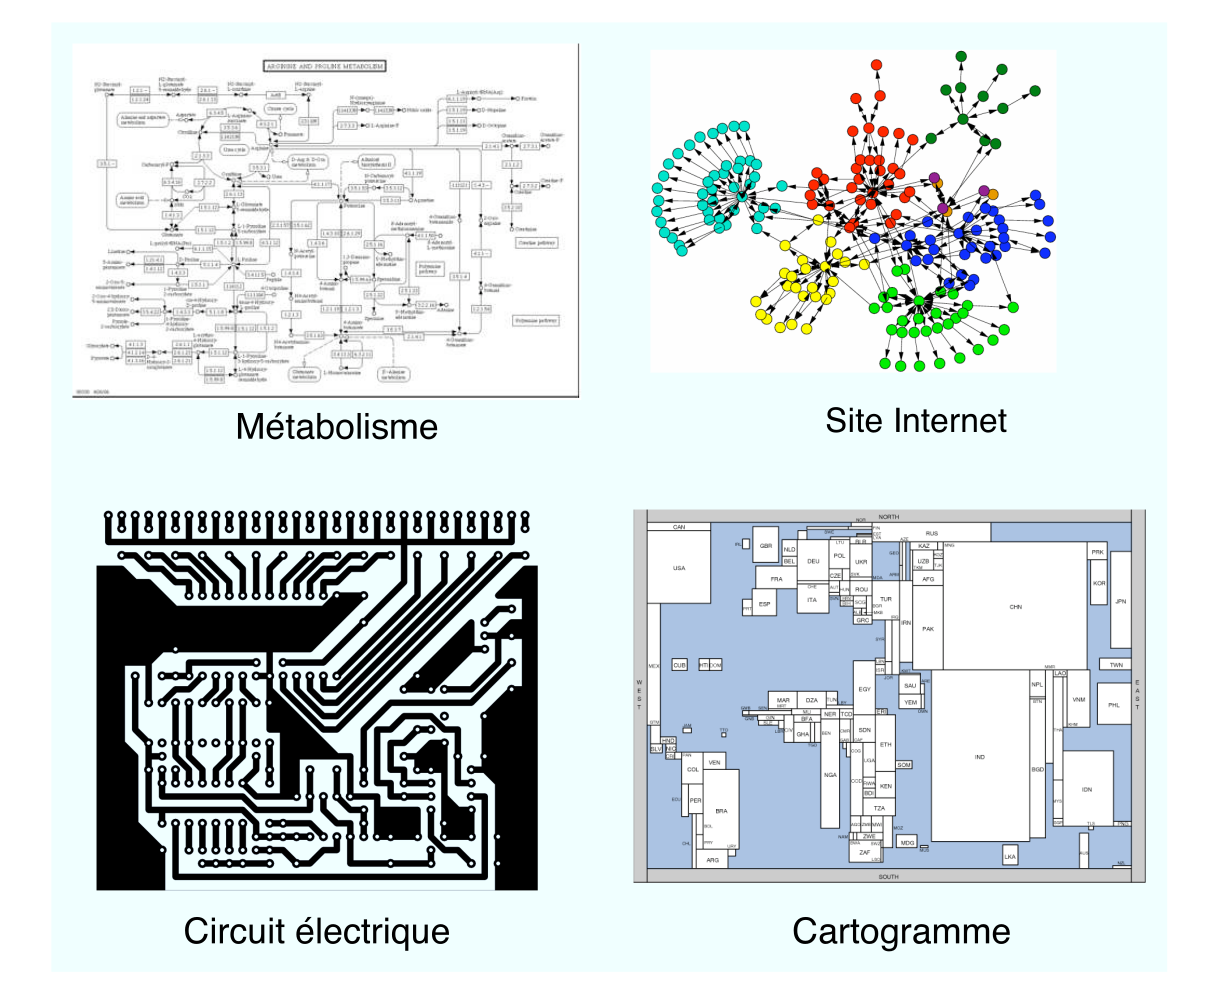
\includegraphics[height=0.86\textheight]{motivation.png}\\[-.2cm]
    \caption[caption]{Cas d'utilisation de graphe.  \\\vspace*{0.1cm} Source: Référence sur le document \citeauthor{fusy2007combinatoire}}	
	\end{figure}
        \end{column}
    \end{columns}

\end{frame}

%%%%%%%%%%%%%%%%%%%%%%%%%%%%%%%%%%%%%%%%%%%%%%%%%%%%%%%%%%%%%%%%%%%%%%%%%%%%%%
%%%%%%%%%%%%%%%%%%%%%%%%%%%%%%%%%%%%%%%%%%%%%%%%%%%%%%%%%%%%%%%%%%%%%%%%%%%%%%

\section[Ordre canonique]{Ordre canonique}
\subsection{Conditions}	
{
\begin{frame}{}
	\begin{block}{Conditions}
		Soit $G = (V, E)$ un graphe planaire triangulé avec $n$ nombre de sommets $3 \le n$. 
		un ordre canonique \(\pi=(v_{1}, v_{2}, \ldots ,v_{n}) \), si les conditions suivantes sont remplies pour chaque $k$, $3 \le k \le n$ :
	\end{block}
\begin{columns}

\begin{column}{0.5\textwidth}
    \begin{minipage}{1\textwidth}
    \begin{block}{}
	  \begin{enumerate}
		\item $\{v_{1}$, $v_{2}\}$ appartient à la face extérieure du $G$; \\[.2cm]		
		\item Les sommets \( (v_1, \ldots ,v_n) \) induisent un graphe $G_{k}$ \textbf{2-connexe} et \textbf{intérieurement triangulé}; \\[.2cm]
 		\item Si \(k+1 < n\), le sommet $v_{k+1}$ se trouve sur la face externe de $G_k$. Et tous les voisins de $v_{k+1}$ apparaissent consécutivement sur la frontière $C_o(G_k)$ \citeauthor{TakaoSaidur}. 
 			%$v_k$ est intégré en un point $\mu(P_1,P_2)$ d'intersection des deux diagonales, la première avec une pente $+1$ passant par $w_p$ et la deuxième avec une pente $-1$ passant par $w_q$ , on a le point :\\ 		 
	  \end{enumerate}
    \end{block}
    \end{minipage}
\end{column}
  
\begin{column}{0.45\textwidth}  %%<--- here
	\begin{figure}
		\centering
		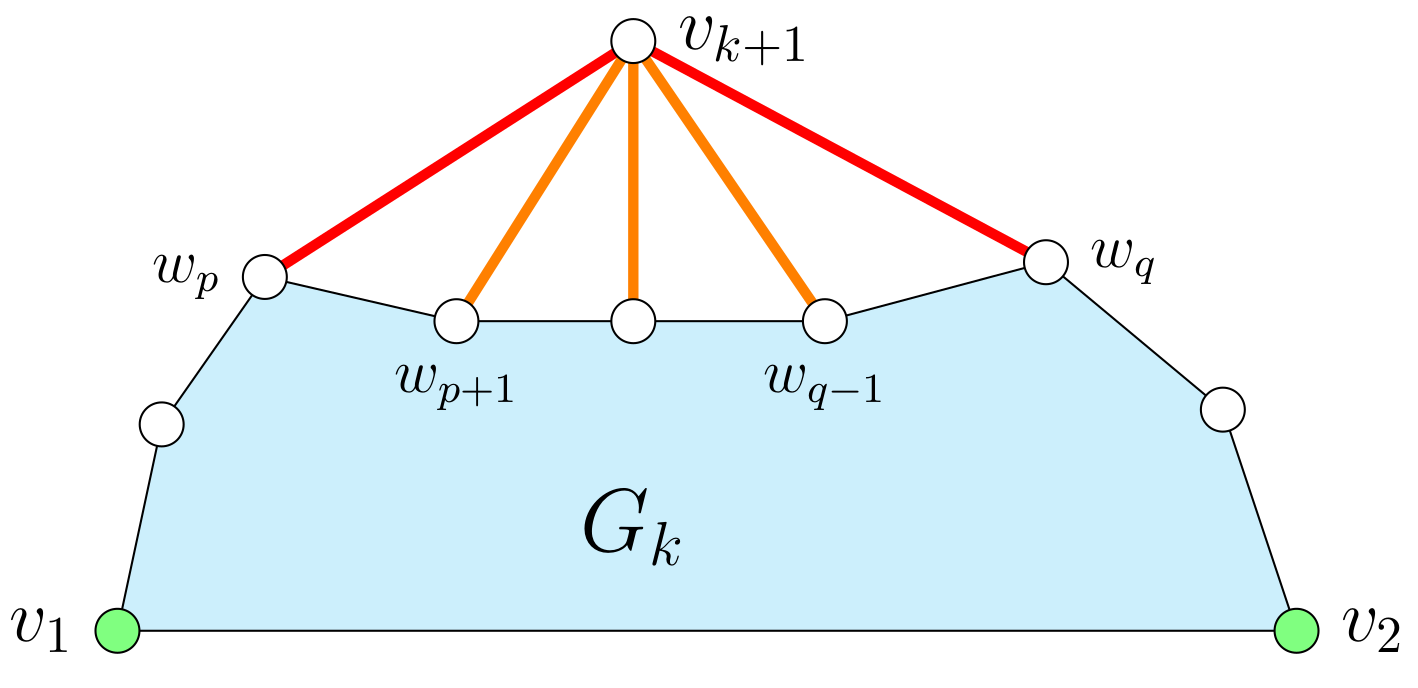
\includegraphics[height=0.27\textheight]{oc0.png}\\[-.2cm]
\caption[caption]{Le choix du sommet $v_k$ pour l'ordre canonique. \\\vspace*{0.1cm} Référence: document \citeauthor{PhilippKindermann}}	
	\end{figure}
\end{column}
\end{columns}	
\end{frame}
}

\subsection{Cas particulier}	
{
\begin{frame}{}
	\begin{figure}
		\centering
		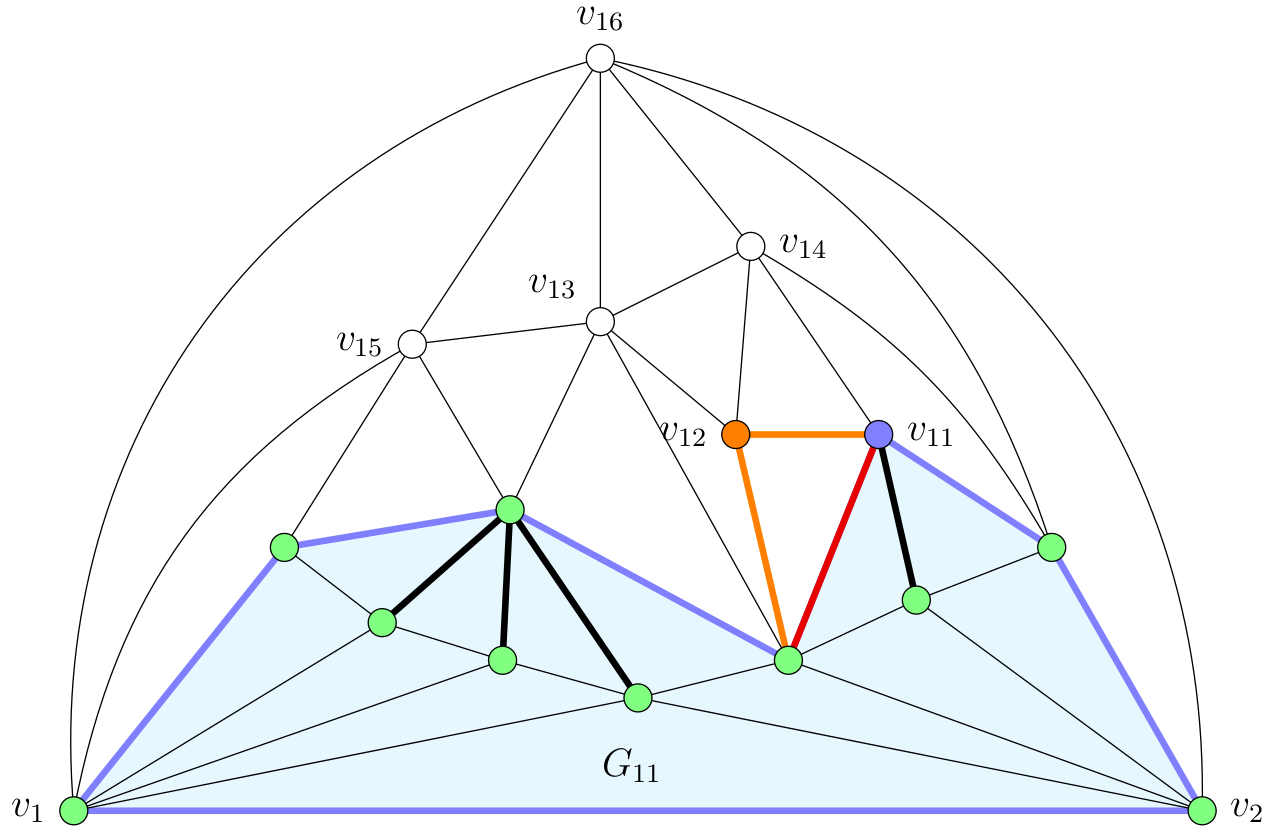
\includegraphics[height=0.7\textheight]{oc2.png}\\[-0.2cm]
\caption[caption]{Le cas d'un corde sur l'ordre canonique. \\\vspace*{0.1cm} Référence: document \citeauthor{PhilippKindermann}}	

	\end{figure}
\\[-0.5cm]
 \centering
\begin{minipage}{0.8\textwidth}
\begin{block}{}
Corde: Arête reliant deux sommets non adjacents dans un cycle.
\end{block}
\end{minipage}

\end{frame}
}
%%%%%%%%%%%%%%%%%%%%%%%%%%%%%%%%%%%%%%%%%%%%%%%%%%%%%%%%%%%%%%%%%%%%%%%%%%%%%%%%%%%%
%%%%%%%%%%%%%%%%%%%%%%%%%%%%%%%%%%%%%%%%%%%%%%%%%%%%%%%%%%%%%%%%%%%%%%%%%%%%%%%%%%%%

\section[Shift Method]{Shift Method}
\subsection{Dessin et Conditions}	
{
\begin{frame}{}
\begin{columns}
	\begin{column}{0.3\textwidth}
 \\[-2.5cm]
\begin{block}{Conditions}
%	\fontsize{6pt}{6pt}\selectfont
	\begin{enumerate}
		\item \footnotesize $v_1$ à (0, 0) et $v_2$ à (2k-6, 0);\\[.5cm]
		\item \footnotesize Chaque sommet de $C_o(G_{k-1}) \setminus \{v_1, v_2\}$ est x-monotone;	\\[.5cm]
		\item \footnotesize Chaque arête de la frontière du $G_{k-1} \setminus \{v_1, v_2\}$ est dessinée avec des pentes de $\pm 1$. 
	\end{enumerate} 
\end{block}	
	\end{column}
	\begin{column}{0.9\textheight}
			\begin{figure}
			\centering
			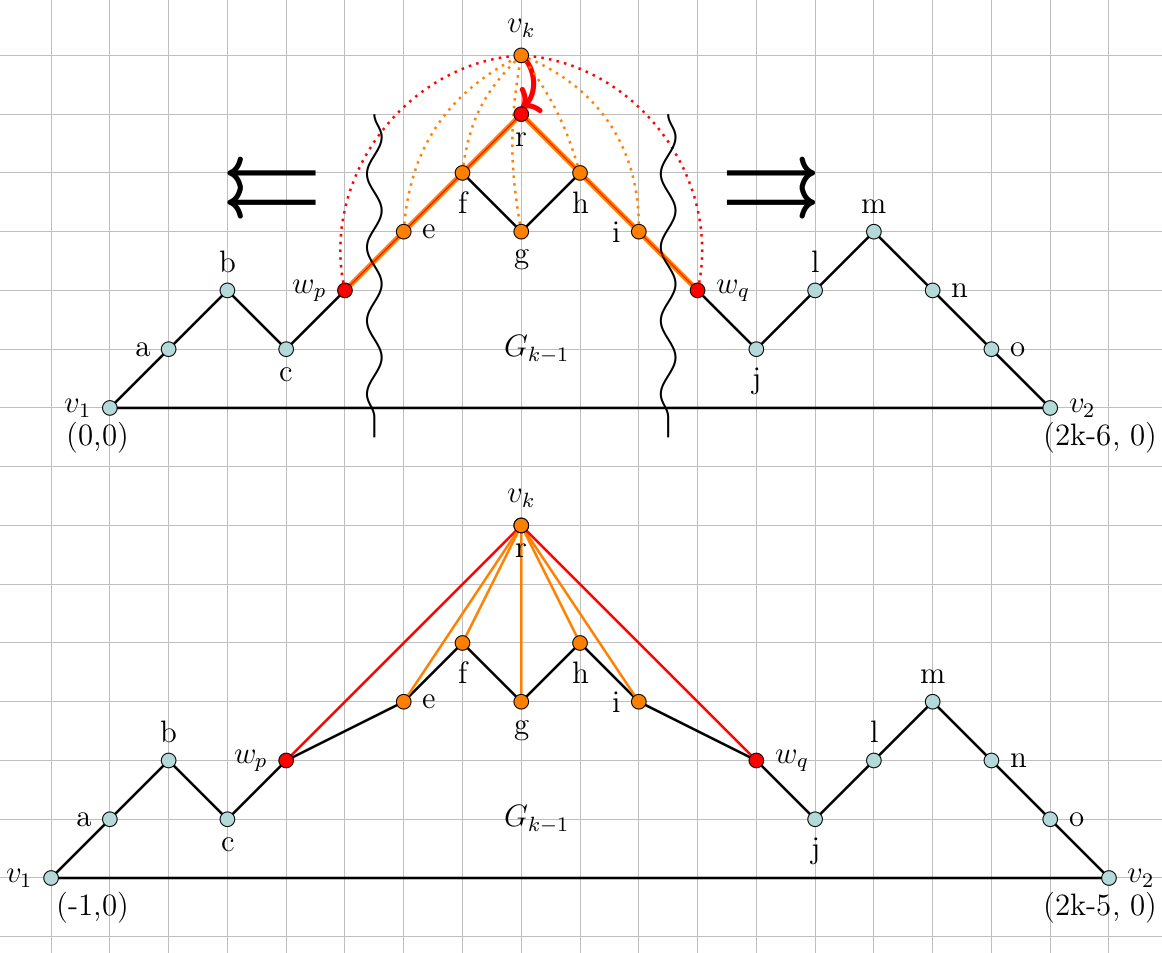
\includegraphics[height=.76\textheight]{sm1.png}\\[-.2cm]
\caption[caption]{Le Graphe avant et après décalage. \\\vspace*{0.1cm} Référence: document \citeauthor{TakaoSaidur}}	   
		\end{figure}
	\end{column}
\end{columns}
	
\end{frame}
}



\subsection{Insertion de prochain sommet $v_k$}	
{
\begin{frame}{}
    \begin{block}{Calcules}
		\begin{enumerate}
			\item $x(v_k) = \frac{1}{2} [ x(w_q) + x(w_p) + y(w_q) − y(w_p)]$
			\item $y(v_k) = \frac{1}{2} [ x(w_q) + x(w_p) + y(w_q) − y(w_p)]$
			\item $x(v_k )-x(w_p) = \frac{1}{2} [ x(w_q)−x(w_p)+y(w_q)-y(w_p)]$ 
		\end{enumerate} 
	\end{block}	

    \begin{figure}
		\centering
		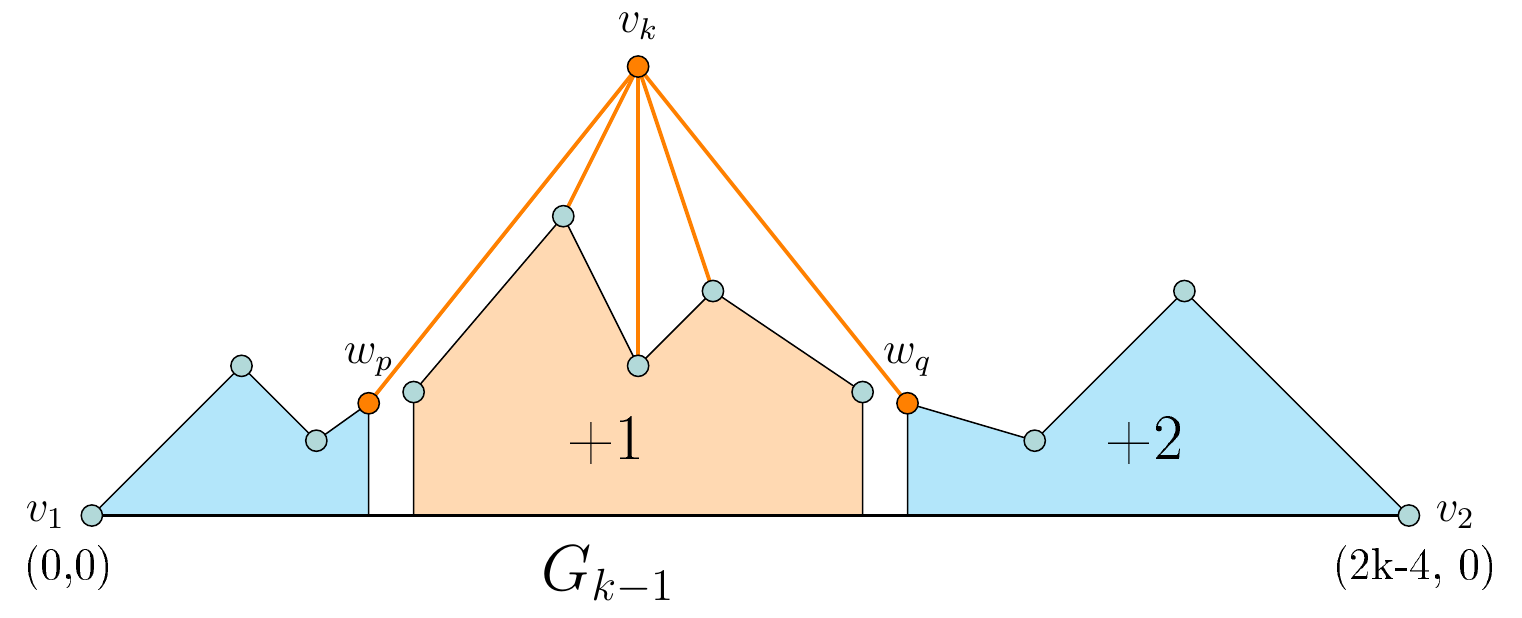
\includegraphics[width=0.8\textwidth]{sm0.png}\\[-.2cm]
    \caption[caption]{Illustration du décalage dans la méthode shift. \\\vspace*{0.2cm} Source: document \citeauthor{PhilippKindermann}}	
	\end{figure}

\end{frame}
}


  
%%%%%%%%%%%%%%%%%%%%%%%%%%%%%%%%%%%%%%%%%%%%%%%%%%%%%%%%%%%%
%%%%%%%%%%%%%%%%%%%%%%%%%%%%%%%%%%%%%%%%%%%%%%%%%%%%%%%%%%%%

\section[Structure de donnée]{Structure de donnée}
\subsection{Arbre} 	
{
\begin{frame}{}

\begin{columns}
    \begin{column}{0.6\textwidth}
    \begin{figure}
		\centering
		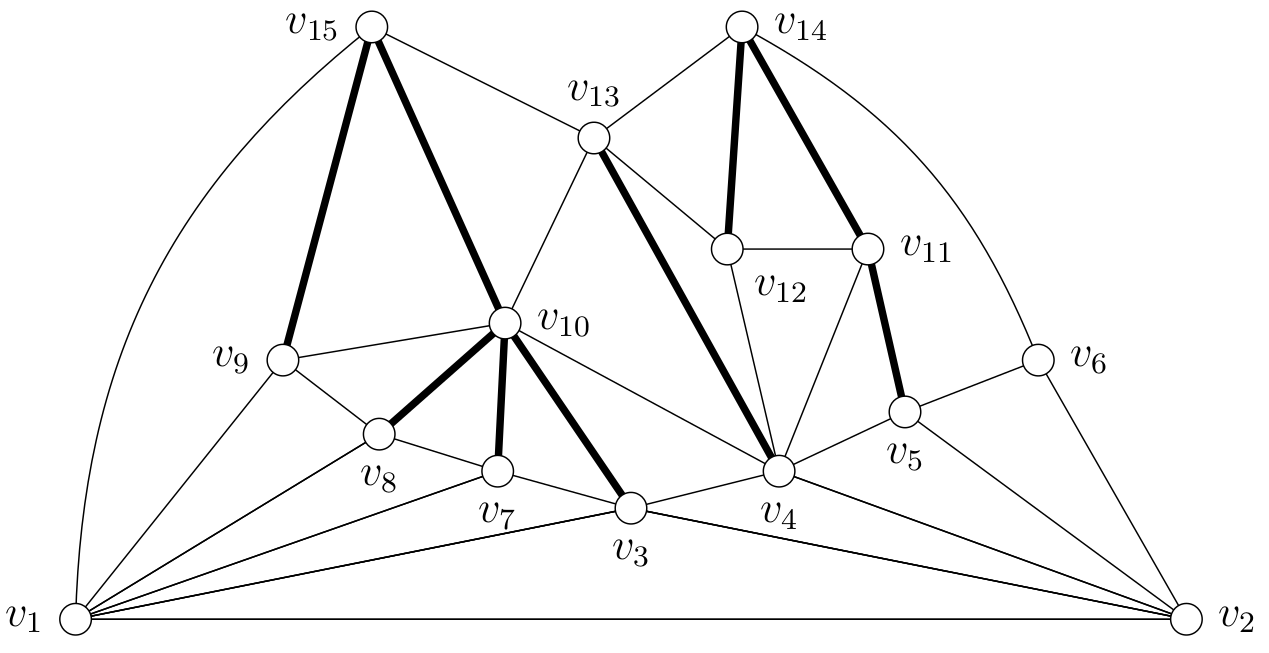
\includegraphics[width=0.9\textwidth]{oc4.png}\\[.1cm]
    \caption[caption]{Ordre canonique de $G_{15}$. \\\vspace*{0.2cm} Référence: document \citeauthor{PhilippKindermann}}	
	\end{figure}
    \end{column}
    
    \begin{column}{0.4\textwidth}
    \begin{figure}
		\centering
		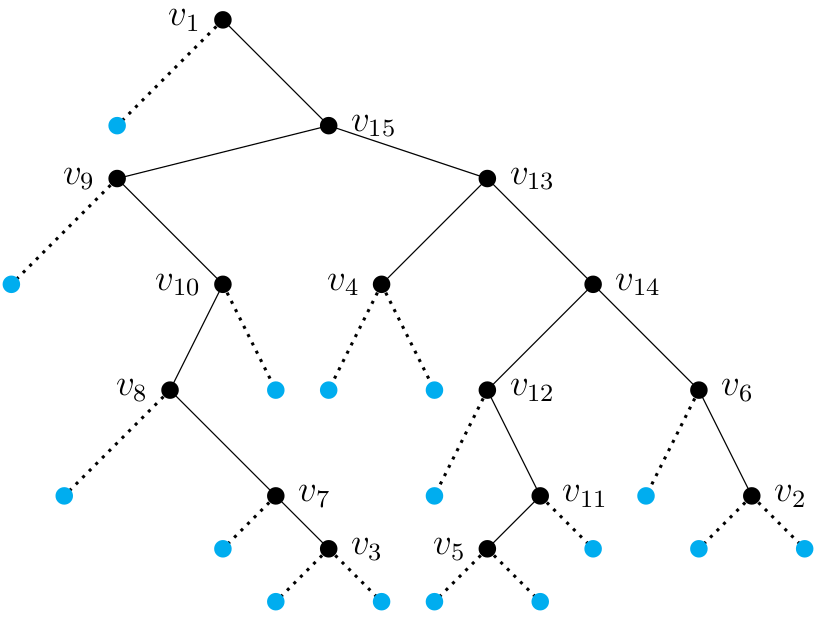
\includegraphics[width=0.9\textwidth]{oc3.png}\\[.1cm]
    \caption[caption]{La forêt $F$ de $G_{15}$. \\\vspace*{0.2cm} Référence: document \citeauthor{PhilippKindermann}}	
	\end{figure}
    \end{column}
\end{columns}  

\centering
\begin{minipage}{0.5\textwidth}
    \begin{block}{}
     \begin{itemize}
		\item \small Fils $gauche(v)$ dans $T$ ; 
		\item \small Fils $droit(v)$ dans $T$ ; 
		\item \small $\Delta x(v) = x(v) - x(w) $ ; 
		\item \small $y(v)$.
    \end{itemize}
    \end{block}
\end{minipage}

\end{frame}	
}

\subsection{Arbre couvrant} 	
{
\begin{frame}{}

    \begin{figure}
		\centering
		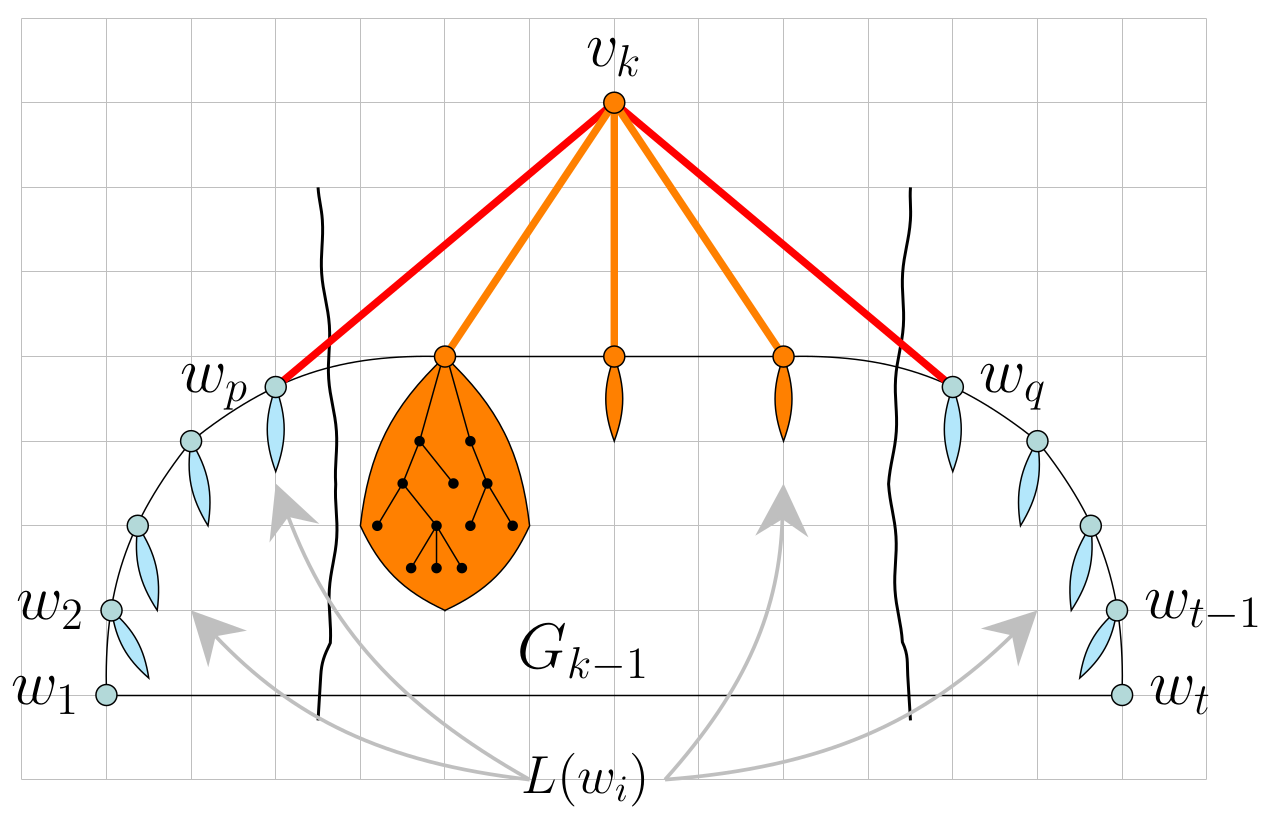
\includegraphics[width=0.45\textwidth]{sd1.png}\\[-.2cm]
    \caption[caption]{Le graphe $G_k$. \\\vspace*{0.1cm} Source: document \citeauthor{PhilippKindermann}}	
	\end{figure}

    \begin{figure}
        \centering
        \includegraphics[width=0.5\textwidth]{com1.png}\\[-.2cm]
		\caption[caption]{(b) l'arbre $T$ du $G_{k-1}$, et (c) l'arbre $T$ du $G_{k}$. \\\vspace*{0.1cm} source:\citeauthor{TakaoSaidur}} 
	\end{figure}
    	
\end{frame}	
}
%%%%%%%%%%%%%%%%%%%%%%%%%%%%%%%%%%%%%%%%%%%%%%%%%%%%%%%%%%%%
%%%%%%%%%%%%%%%%%%%%%%%%%%%%%%%%%%%%%%%%%%%%%%%%%%%%%%%%%%%% 
  
\section{Algorithme Shift method}	
\subsection{Algorithme Shift method}	
{
\begin{frame}[allowframebreaks]{}
\fontsize{9pt}{10pt}\selectfont
\\[-.3cm]
%\begin{algorithm}[H]
%\footnotesize
%\fontsize{9pt}{9pt}\selectfont %Frame with different font sizes and spacing
%\caption{\footnotesize Shift method}
\rule{\textwidth}{0.5pt}
\vspace*{-0.4cm}
\captionof{algorithm}{\footnotesize Shift method}%
\vspace*{-0.4cm}
\rule{\textwidth}{0.5pt}%
\vspace*{0.1cm}

\begin{algorithmic}[1]
\INPUT{Graphe planaire $G$ à n sommets, et son ordre canonique}
\OUTPUT{Dessin planaire en line droite du $G$ sur une grille $(2n−4) \times (n−2)$}
\Statex Soit $v_1, \dots, v_n$ l'ordre canonique du graphe $G$;	
\Statex Soit $w_1, w_2,\dots, w_t$ le $C_o(G_{k-1})$ de $G_{k-1}$;
\Statex Soit \(w_p, w_{p+1},\dots, w_q\) les voisins de $v_k$ sur $C_o(G_{k-1})$;

\State $ (\Delta x(v_1), y(v_1), gauche(v_1), droit(v_1)) = (0, 0, null, v_3) $; \Comment{Initialisation}
\State $ (\Delta x(v_3), y(v_3), gauche(v_3), droit(v_3)) = (1, 1, null, v_2) $;
\State $ (\Delta x(v_2), y(v_2), gauche(v_2), droit(v_2)) = (1, 0, null, null) $;
\For {$4 \le k \le n$}  
\State $ \Delta x(w_{p+1}) = \Delta x(w_{p+1})+1 $ ; \Comment{Augmenter le décalage de $w_{p+1}$ de 1}
\State $ \Delta x(w_{q}) = \Delta x(w_{q})+1 $ \Comment{Augmenter le décalage de $w_q$ de 1}

\State $ \Delta x(w_p,w_q) = \Delta x(w_{p+1}) +....+ \Delta x(w_q) $; \Comment{$\mathcal{O}(d(v_k))$}
\State $ \Delta x(v_k) = \frac{1}{2}[\Delta x(w_p,w_q) + y(w_q) - y(w_p)] $ ; \textit{cf.}(4);
\State $ y(v_k) = \frac{1}{2}[\Delta x(w_p,w_q) + y(w_q) + y(w_p)] $ ;  \textit{cf.}(3);

\State $ \Delta x(w_q) = \Delta x(w_p,w_q) - \Delta x(v_k) $; \Comment{Ajuster le décalage de $w_{q}$ }

\If{$ (p + 1) \neq q $}
    \State $ \Delta x(w_{p+1}) = \Delta x(w_{p+1}) - \Delta x(v_k) $;
    \EndIf
\State $ droit(w_p) = v_k $ et $ droit(v_k) = w_q $ ; \Comment{Insertion  de $v_k$}

\Statex 
\Statex \Comment{À suivre}


\If{$ (p + 1) \neq q $}
    \State  $ gauche(v_k) = w_{p+1} $ et $ droit(w_{q-1}) = nil $;
\Else 
    \State $ gauche(v_k) = nil $;
	\EndIf
\EndFor

\State $x(v_1) = 0$;
\State AccumulateOffset(v_1 ,x(v_1)); \Comment{$\mathcal{O}(n)$}

\end{algorithmic}
%\end{algorithm}


\begin{algorithm}[H]
\caption{Procedure AccumulateOffset}
\begin{algorithmic}[1]
\INPUT{($v$: sommet ; $\delta$: entier)}
      \If{$ v \neq null $}
        \State $\Delta (v) = \Delta (v) + \delta $
        \State Accumulate-Offset$(gauche(v), \Delta x(v))$ 
        \State Accumulate-Offset$(droit(v), \Delta x(v))$
		\EndIf
\end{algorithmic}
\end{algorithm}


\end{frame}
}

%%%%%%%%%%%%%%%%%%%%%%%%%%%%%%%%%%%%%%%%%%%%%%%%%%%%%%%%%%%%
%%%%%%%%%%%%%%%%%%%%%%%%%%%%%%%%%%%%%%%%%%%%%%%%%%%%%%%%%%%%

\section[Conclusion]{Conclusion}

\begin{frame}{Conclusion}
\begin{itemize}
	\item Shift method, \citeauthor{FraysseixPachPollack} offre une approche efficace pour créer des représentations visuelles claires et ordonnées
de ces graphes. \\[.2cm]
    \item Compréhension de la représentation en ligne droite des graphes planaires. \\[.2cm]
    \item Visualisation et l’analyse de ces graphes
    \item Un temps d'exécution en $\mathcal{O}(n)$ en temps et en espace.\\[.2cm]    
    \item Plus grande quantité de données.

	\end{itemize}
	
\end{frame}	
%%%%%%%%%%%%%%%%%%%%%%%%%%%%%%%%%%%%%%%%%%%%%%%%%%%%%%%%%%%%
%%%%%%%%%%%%%%%%%%%%%%%%%%%%%%%%%%%%%%%%%%%%%%%%%%%%%%%%%%%%

\section[Application]{Application} 
\subsection{Bases de données orientées graphe}
\begin{frame}{}
    \centering
    \begin{columns}
    \begin{column}{0.4\textwidth}
        \begin{minipage}{0.9\textwidth}
        \begin{block}{}
        - Une grande importance entre les liens. \\[.2cm]
        - Les relations sont stockées nativement. \\[.2cm]
        - Tout est un graphe de relations interconnectées.\\[.2cm]
        - Parcourir rapidement les données; des millions de connexions par seconde, par cœur.\\[.2cm]
        Source : \url{https://neo4j-com}
        \end{block}
        \end{minipage}
    \end{column}
        
\begin{column}{0.6\textwidth}
        \begin{figure}
		\centering
		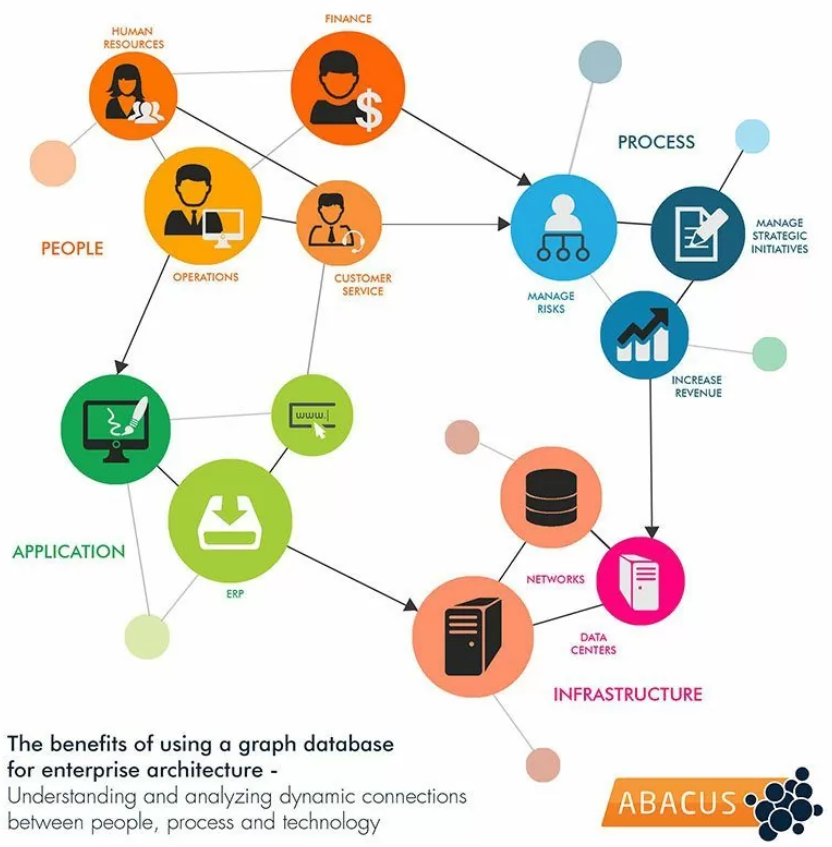
\includegraphics[height=0.8\textheight]{moti1.png}\\[-.2cm]
\caption[caption]{Exemple d'une base de donnée orientée graphe. \\\vspace*{0.1cm} Référence: \url{https://www.avolutionsoftware.com/}}	
	\end{figure}
\end{column}
\end{columns} 

\end{frame}

%%%%%%%%%%%%%%%%%%%%%%%%%%%%%%%%%%%%%%%%%%%%%%%%%%%%%%%%%%%%
%%%%%%%%%%%%%%%%%%%%%%%%%%%%%%%%%%%%%%%%%%%%%%%%%%%%%%%%%%%%
\section[Annexe]{}
\begin{frame}[plain,noframenumbering]{Annexe}
	
	Toutes les sources et l’intégralité de ce code qu'ont servi à la rédaction de cette présentation se trouvent sur le document latex sur ce lien : \\[.5cm]
	\url{https://github.com/Kazzoul-Youness/StraightLine-ShiftMethod}
	
\end{frame}

%%%%%%%%%%%%%%%%%%%%%%%%%%%%%%%%%%%%%%%%%%%%%%%%%%%%%%%%%%%%%%%%%%
\section[Références]{}
\begin{frame}[plain,noframenumbering]{Références}
	\bibliographystyle{apalike}
	\bibliography{ref.bib} 	
\end{frame}

%%%%%%%%%%%%%%%%%%%%%%%%%%%%%%%%%%%%%%%%%%%%%%%%%%%%%%%%%%%%%%%%%%
\section[Questions]{}
\begin{frame}[plain,noframenumbering]{Questions}
	\begin{center}
		Questions 
	\end{center}
\end{frame}	

%%%%%%%%%%%%%%%%%%%%%%%%%%%%%%%%%%%%%%%%%%%%%%%%%%%%%%%%%%%%%%%%%%

\end{document}
